\documentclass{acm_proc_article-sp}
\usepackage{breqn}
\usepackage{caption}
\usepackage{hyperref}
\usepackage[all]{hypcap}
\usepackage{subfig}
\makeatletter
\def\@copyrightspace{\relax}
\makeatother

\title{An Analysis of Shared Library Performance \\ on NUMA Architectures}

%\author{Neeraj Kumar,˜\IEEEmembership{University of Waterloo }
%	Hemant Saxena,˜\IEEEmembership{University of Waterloo} }

\numberofauthors{2}
\author{
Neeraj Kumar\\
neeraj.kumar@uwaterloo.ca
\alignauthor
Hemant Saxena
hemant.saxena@uwaterloo.ca
}

\begin{document}

\maketitle

\subsection*{Abstract}

Most modern multicore systems these days are Non Uniform Memory Architecture (NUMA), which means they have multiple memory controllers
with non-uniform access latencies across them. There has been significant amount of work done in exploring and 
mitigating performance penalty due to NUMA overhead. In previous works, NUMA-aware schedulers were proposed,
sometimes with an objective of keeping data close to the processors working on them and sometimes to attain a 
trade-off between data locality and cache contention. \\
However, the effect of instructions on process' performance in context of NUMA has not been explored yet.
In this work, we present an analysis about the performance hit on processes due to instructions on NUMA machines.
We limit our focus to the impact of shared code, which by definition has a single copy and resides on one of the NUMA nodes.
We also discuss various scenarios in which a single copy of these shared objects can harm the performance due to remote
fetches and present some ideas to alleviate the problem.



\section{Introduction}

With the constantly increasing number of cores in modern multicore systems, Non-uniform memory architectures
are becoming more and more common. In its simplest form, a NUMA can have two processors with local memories connected
to each other via an interconnect. Naturally, access to local memory is faster than the remote by a factor greater than 1,
called the numa factor or numa overhead. With more processors, the interconnections become more complex, and the numa factor
can also be different for different pair of nodes.

With the introduction of NUMA architectures, problems with respect to data locality becoming bottleneck for application performance
has drawn significant academic attention. Previous work by Brecht\cite{Brecht:1993:IPA:1295480.1295481} and 
Broquedis et al.\cite{numaScheduling} explore placement decisions in context of data locality.
In another recent work \cite{Dashti:2013:TMH:2490301.2451157}, the authors claim that contrary to older systems,
modern NUMA hardware has much smaller remote wire delays, and so remote access costs per se are not the main 
concern for performance, instead, congestion on memory controllers and interconnects, caused by memory traffic 
from data-intensive applications, hurts performance a lot more.

Another work by Majo et. al. \cite{Majo:2011:MMN:1993478.1993481} tends to exploit the trade-off between cache contention
and interconnect overhead while scheduling threads on NUMA machines. Running two threads of a process on the same socket
avoids interconnect overhead but experiences a penalty in terms of cache contention, as last level cache are shared for
threads running on the same socket, Whereas scheduling two threads on different sockets can avoid cache contention
as two threads will use their local LLCs but the penalty of data fetch over interconnect can hit the performance in this case.
Majo et. al. \cite{Majo:2011:MMN:1993478.1993481} have introduced N-MASS algorithm, which is a cache conscious scheduler for NUMAs.

The problems addressed in previous works mainly deal with the data-section associated with the program. We believe that
a similar problem exists for text-section of the program in context of NUMA environment, albeit less aggravated
because of the text-section being read-only. In this work, we present a detailed analysis for this problem in context of
shared libraries, which by definition has a single copy across all memory nodes, and is loaded into memory when an object
linked against it starts execution.

Text-section of a program mostly consists of instructions and read-only global data. In case of shared libraries, this section
is unique across all memory nodes and will be shared by all the running processes linked against that library. As the text
section is read-only and would be rarely evicted, it makes sense to have an extra cache for instructions. This is accomplished
by having instruction only caches at L1 level, called L1-icache. Normally, as code size is dependent upon the program complexity,
which is fixed, this means that the growth is not as bad as in case of data. Additionally, program flow being more predictable
than data access patterns, it is normally the case that active code can somewhat fit in the cpu caches.
However, it is still not uncommon to find applications using big shared libraries. In cases when the size of shared library exceeds
the cache-sizes or for some reason prefetching fails, the instructions will need to be fetched from the main memory.
This can result in two problems, increased latencies due to instructions being fetched from remote node and increased overhead on
memory controllers and interconnects due to congestion. In this work, we examine and analyze the cost of code on a remote NUMA
node from both these perspectives and discuss the results. We also discuss some ideas that can be applied to mitigate the problem.

The remainder of the paper is organized as follows. In the next section, we discuss a little bit about shared libraries and 
then talk about our experimental setup. In section 3, we will discuss at length the motivation, results and also the explanation
of the results for each of the experiments performed. In section 4, we will discuss about some ideas that could potentially improve
the system performance with shared libraries on NUMA machines and talk about the road map to their implementation in future works.
Finally we conclude, highlighting the key observations from our experiments.



%\section{NUMA}
%\begin{figure}
    \centering
    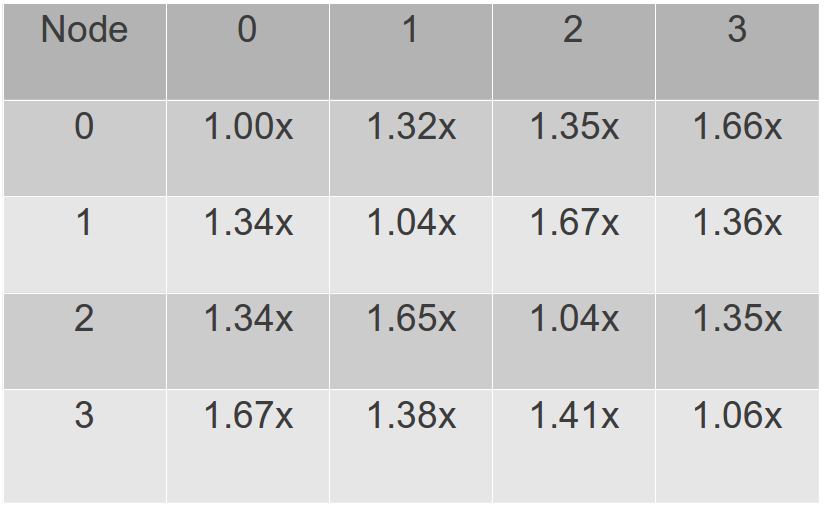
\includegraphics[scale=0.35]{numaMatrix.png}
    \caption{This shows the slowdown between each node. }
    \label{fig:numaMatrix}
\end{figure}



\section{Shared Library}

Shared libraries are basically object files, that are loaded, (if not already) at runtime
when a process linked against it starts execution. The pages remain in the memory until
they are swapped out by pages from another program, based upon the page replacement algorithms\cite{pageReplacement}.

Shared libraries are useful because of multiple reasons. They allow programmers to make use of existing
code without increasing the executable sizes. Additionally, as there is a single copy of shared code, there
are fewer page faults because its possible that some other process may have already loaded the shared code.
In addition to this, shared libraries also make it easy to upgrade to newer versions of the code.

\begin{figure}
    \centering
    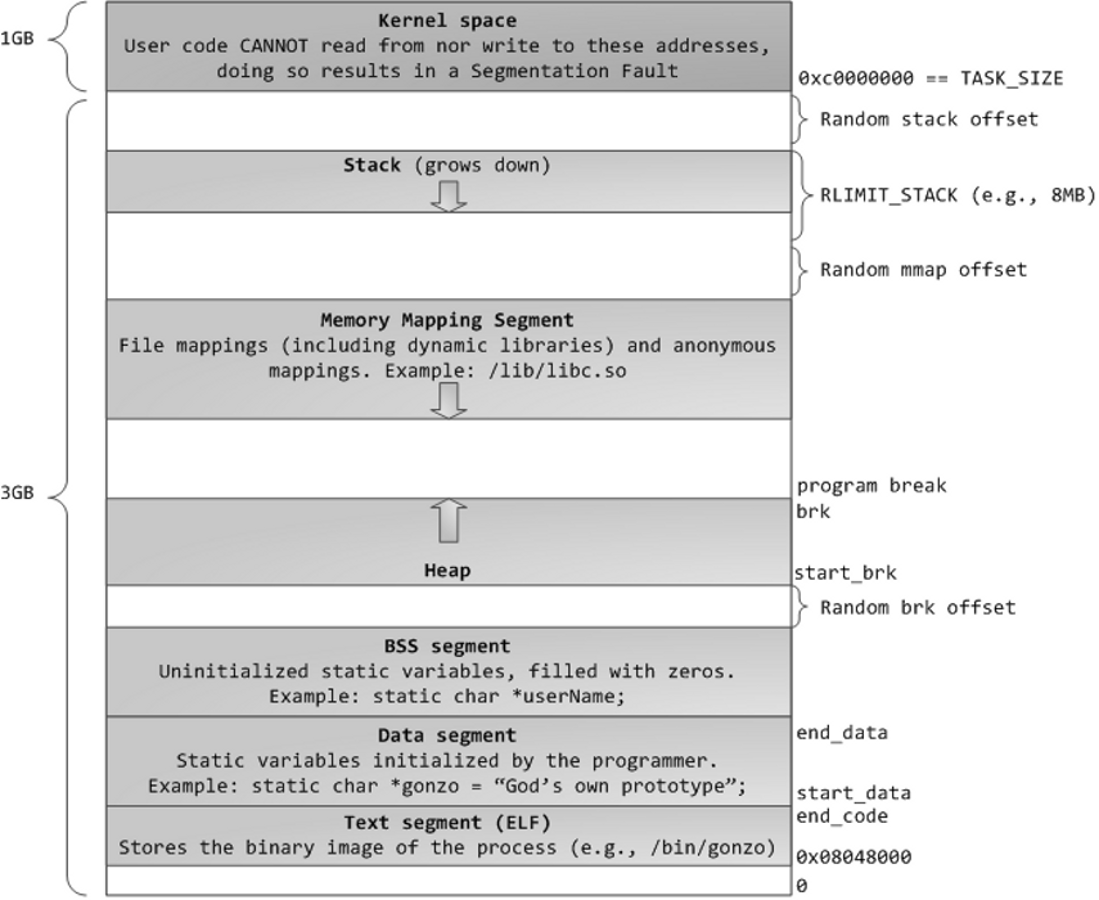
\includegraphics[width=\linewidth, height=8.5cm]{linuxFlexibleAddressSpaceLayout.png}
    \caption{Anatomy of a program in memory, Image Source:\cite{anatomyOfProgramInMemory}}
    \label{fig:processInMemory}
\end{figure}

Figure \ref{fig:processInMemory} shows how a running program looks like in the memory. Shared libraries, can be
loaded elsewhere in the memory, and the address mappings are stored in the memory mapping segment.
Size of a shared library depends upon the text-section, (which is mostly the shared-code and read-only data) and
the data and bss sections, which correspond to global and uninitialized data respectively. Figure \ref{fig:sizeOutput}
shows the result of \textit{size} command on the libnuma shared library. It can also be seen that, most of the shared
libraries on a normal linux-like systems are small, that is, less than 2 MBs. As such, they can easily fit in the
processor caches, and performance impact due to NUMA overhead would be negligible. However, some shared libraries
are big, (figure \ref{fig:libSizes} lists some big libraries) and we may have even bigger libraries in future.
Therefore, it is worthwhile to evaluate the performance impact in context of NUMA machines and perform possible
optimizations.

\begin{figure}
    \centering
    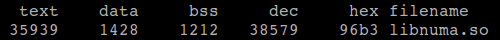
\includegraphics[width=\linewidth]{sizeOutput.png}
    \caption{output of \textit{size} command on libnuma.so}
    \label{fig:sizeOutput}
\end{figure}

\begin{figure}
    \centering
    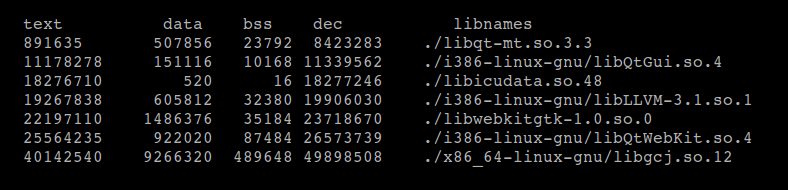
\includegraphics[width=\linewidth, height=2.5cm]{libSizes.png}
    \caption{Sizes for some big libraries}
    \label{fig:libSizes}
\end{figure}


\section{Experimental Setup}

All our experiments were performed on a NUMA machine with 4-sockets each housing a six-core AMD Opteron 8431 processor \cite{opteron}.
Cache related and topology related information about the NUMA hardware can be found at:

\texttt{/sys/devices/system/cpu/cpu*/cache } \\
\\
\texttt{ /sys/devices/system/cpu/cpu*/topology }

The L1, L2 and L3 sizes for the machine were 128, 512 and 6144 KBytes respectively.

\subsection{Performance monitoring}
For our measurements, we relied on \texttt{RDTSC} assembly instruction\cite{timeStampCounter} for getting CPU timing information
and \texttt{perf stat} \cite{perfWiki}, for counting the cache misses, page-faults and stalled CPU cycles. We used libnuma,
the NUMA policy library, for control and placement of threads and data on the NUMA nodes. \cite{libNuma} lists many functions
that can be used to modify the default numa policy as required. The command line interface, \texttt{numactl} \cite{numactl} 
provides various command-line arguments like \texttt{cpubind} and \texttt{membind} to bind processes and data to specific nodes.

\subsection{Interconnect Overhead}
Shared code is in essence very similar to read-only data, unless it is self-modifying.
Therefore, all the observations with respect to NUMA overheads for read-only data can be generalized for shared code as well.
In this section, we compute the overhead of fetching the data over the interconnect by comparing the access times for read-only
data for local and remote memory access.

To make our measurements more accurate, we undermine the effect of cpu caches by flushing the cache line associated with the 
variable before every memory access. We do this by using the CLFLUSH\cite{clflush} assembly instruction as follows.
\begin{verbatim}
// ...
const char* roData = "foo";
clflush(roData);
tmp = *roData;
// ...
\end{verbatim}

It should be noted that, if the cpu cache is flushed before the computation, the total ticks elapsed will be the sum of time 
taken to fetch the operand from memory and execute the instruction.
\begin{dmath}
\label{eqn:NoCacheFetch}
T_{CFlush} = T_{MemFetch} + T_{decodeAndExecute}
\end{dmath}

Whereas, if the cache is not flushed, the data is too small and can easily fit in L1 cache, therefore, 
\begin{dmath}
\label{eqn:cacheFetch}
T_{NoCFlush} \approx T_{decodeAndExecute}
\end{dmath}

From \ref{eqn:NoCacheFetch} and \ref{eqn:cacheFetch}, we can compute the value for $T_{MemFetch}$, the
results for which are labeled in the following table (all entries in clock ticks):

\begin{center}
\begin{tabular}{c|c|c|c}
\hline
location & T_{CFlush} & T_{NoCFlush} & T_{MemFetch}\\
\hline
Self & 944 & 330 & 614\\
Horizontal & 1262 & 330 & 932 \\
Vertical & 1258 & 330 & 928\\
Diagonal & 1570 & 330 & 1240\\
\hline
\end{tabular}
\end{center}

From the table above, it can be concluded that adjacent access is 1.5x costly whereas diagonal access is
2x costlier. These observed results agree with the fact that for 4-node NUMA machines, the topology is
hypercube with \textit{C} = 2, as discussed here\cite{Drepper07whatevery}.



\section{Analysis} \label{sec:analysis}
\subsection{Remote vs Local Library}
In the above section we saw the interconnect overhead in terms of slowdown, when we try to fetch data from remote node.
Similar overhead exist in the case when read-only data is being fetched from remote node.
Here our read-only data is the shared library's instructions.
The shared library was placed on Node03 and then we ran the main thread on each of the four nodes.
Main thread called 0.1 million functions from the library in sequential order.
Figure XX shows the result.
We measured the total number of CPU cycles consumed, stalled cycles and page faults in each case.
We observed that in the case when our main thread was running locally (i.e. on Node03) minimum number of CPU cycles were consumed, and stalled cycles were also minimum.
We measured page faults to make sure that we are fetching equal number of library pages in all four cases, and number of page faults were equal in all four cases.



\section{Future Work} \label{sec:future-work}

Having analyzed the impact of shared code from the perspective of locality and congestion,
we are in a position to suggest some potential improvements that can help to mitigate the
overheads due to NUMA architecture in context of shared libraries.

The default NUMA scheduler currently loads the shared library on the node that triggered
the page-fault for the first library page, which is random. It can be on any of the NUMA nodes.
Such an algorithm is speculative, in the sense that, it expects in future, there may be processes
closer to this node which may potentially use this shared library, and the amortized performance
penalty is not much. However, this may penalize the currently executing program, in case the library
is not loaded on the local node. There are some alternatives, in which we can certainly do better
than the default library placement.

\textbf{Performance-aware loading} Whenever a program executes, first of all the dynamic loader is
invoked with task to load all the shared libraries the program was linked against (if not already loaded).
The programmer knows which all cores he is going to use, for example, if the programmer uses cores from 
two of the four sockets, and the shared library was not already loaded, it seems reasonable to load
the shared library on one of the two nodes. Programmer can explicitly request such a loading or the
compiler may identify this during code analysis, and add relevant information in the binary. This
algorithm comes with almost no overhead, just a slight optimization to make the loader NUMA-aware.

\textbf{User text Replication} Another plausible alternative is replication, which is essentially making
additional copies of the text-section, so that no access for instruction needs to go over the interconnect.
The solution sounds great as it completely eliminates the NUMA overhead but it should be noted that it has
its own costs. It introduces a new problem of keeping all replicated copies in sync, which is a less severe
problem for shared code as it is read-only. The kernel will however, still need to sync every node if any 
of them undergo a page-fault. The advantage being, the system can be implemented transparently in the
kernel and the programmer doesn't has to know about it.

\textbf{Distributed Loading} Another possible solution is loading parts of shared library across all the
NUMA nodes. Such a solution will prevent shared library from becoming a traffic hot-spot and also amortize
the cost of remote NUMA access. The system however will be more complicated as the kernel will need to
keep track of pages on both remote and local nodes and seems worthwhile only if the benefits outnumber the
complexities.

In our future works, we aim to further explore these ideas and implement some of these and present the
outcome of our implementations and how they fare with the challenges presented in this work. One possible
direction of our work can be to use \textit{carefour} \cite{Dashti:2013:TMH:2490301.2451157}, and possibly 
apply their solution in context of shared libraries, as they seem to address similar set of problems.



\section{Related Work}
The work done by Brecht \cite{Brecht:1993:IPA:1295480.1295481} explains that in the case of NUMA scheduler the question of which processor becomes more important than how many processors to be assigned for a task.
His results have shown thread placement decision is critical in large scale multiprocessors.
Work done by Broquedis et al \cite{numaScheduling} is also on the similar lines and talks about dynamic task and data placement over NUMA architecture.
In another recent work \cite{Dashti:2013:TMH:2490301.2451157}, the authors claim that contrary to older systems, modern NUMA hardware has much smaller remote wire delays, and so remote access costs should not be the main concern for performance, instead, congestion on memory controllers and interconnects, caused by memory traffic from data-intensive applications, hurts performance a lot more.
Majo et. al. \cite{Majo:2011:MMN:1993478.1993481} have exploited the trade-off between cache contention and interconnect overhead for their NUMA aware scheduler.



\section{Conclusion} \label{sec:conclusion}

In this paper, we presented a comprehensive analysis of shared library performance
on NUMA architectures. We begin by stating possibility of a performance hit but based
on the results from our experiments, we can conclude that the effect of NUMA overhead
due to non-locality of memory is not as pronounced for shared-code as it is for data.
This is primarily because shared-code is read-only, and therefore exhibits better cache
usage. Based on our experiments, we found that for zipf distribution, 
(which most closely resembles the practical case) the
performance overhead in worst case was found to be about 11\%.
This was when library and thread were scheduled on farthest nodes. We also found that
NUMA overhead increases with increasing library sizes but never exceeds 15\% worst
case overhead.

We also found that when multiple threads concurrently try to access the shared-code,
the performance drops and keeps on dropping linearly as more threads are added to the
system. With 24 threads accessing the library concurrently, the overhead due interconnect
congestion, is as much as 5x times the single-thread case. This is in agreement to the
observation by Dashti et al.\cite{Dashti:2013:TMH:2490301.2451157}, that interconnect congestion
due to multiple threads accessing the data can hurt the performance more than NUMA penalty
would.

To address both these problems together, page replication happens to be the best solution.
We have also discussed couple of other solutions that can possibly improve performance, by
solving one or both of these problems. In our future works, we plan to explore these ideas
further and come up with a working solution.


\bibliographystyle{abbrv}
\bibliography{project}

\end{document}
